%%%%%%%%%%%%%%%%%%%%%%%%%%%%%%%%%%%%%%%%
% datoteka diploma-FRI-vzorec.tex
%
%POZOR: ta verzija ne producira pdf datoteke v pdf/A formatu!!!
%namenjena je le za nalogo pri Diplomskem seminarju!
%
% vzorčna datoteka za pisanje diplomskega dela v formatu LaTeX
% na UL Fakulteti za računalništvo in informatiko
%
% na osnovi starejših verzij vkup spravil Franc Solina, maj 2021
% prvo verzijo je leta 2010 pripravil Gašper Fijavž
%
% za upravljanje z literaturo ta vezija uporablja BibLaTeX
%
% svetujemo uporabo Overleaf.com - na tej spletni implementaciji LaTeXa ta vzorec zagotovo pravilno deluje
%

\documentclass[a4paper,12pt,openright]{book}
%\documentclass[a4paper, 12pt, openright, draft]{book}  Nalogo preverite tudi z opcijo draft, ki pokaže, katere vrstice so predolge! Pozor, v draft opciji, se slike ne pokažejo!
 
\usepackage[utf8]{inputenc}   % omogoča uporabo slovenskih črk kodiranih v formatu UTF-8
\usepackage[slovene,english]{babel}    % naloži, med drugim, slovenske delilne vzorce
\usepackage[pdftex]{graphicx}  % omogoča vlaganje slik različnih formatov
\usepackage{fancyhdr}          % poskrbi, na primer, za glave strani
\usepackage{amssymb}           % dodatni matematični simboli
\usepackage{amsmath}           % eqref, npr.
\usepackage{hyperxmp}
\usepackage[hyphens]{url}
\usepackage{csquotes}
\usepackage[pdftex, colorlinks=true,
						citecolor=black, filecolor=black, 
						linkcolor=black, urlcolor=black,
						pdfproducer={LaTeX}, pdfcreator={LaTeX}]{hyperref}

\usepackage{color}
\usepackage{float}
\usepackage{soul}
\usepackage{listings}
\usepackage[
backend=biber,
style=numeric,
sorting=nty,
]{biblatex}


\addbibresource{literatura.bib} %Imports bibliography file


%%%%%%%%%%%%%%%%%%%%%%%%%%%%%%%%%%%%%%%%
%	DIPLOMA INFO
%%%%%%%%%%%%%%%%%%%%%%%%%%%%%%%%%%%%%%%%
\newcommand{\ttitle}{Upravljanje z identitetami}
\newcommand{\ttitleEn}{Diploma thesis template}
\newcommand{\tsubject}{\ttitle}
\newcommand{\tsubjectEn}{\ttitleEn}
\newcommand{\tauthor}{David Konc}
\newcommand{\tkeywords}{računalnik, identitete, upravljanje, varnost}
\newcommand{\tkeywordsEn}{computer, identity, management, security}

%%%%%%%%%%%%%%%%%%%%%%%%%%%%%%%%%%%%%%%%
%	HYPERREF SETUP
%%%%%%%%%%%%%%%%%%%%%%%%%%%%%%%%%%%%%%%%
\hypersetup{pdftitle={\ttitle}}
\hypersetup{pdfsubject=\ttitleEn}
\hypersetup{pdfauthor={\tauthor}}
\hypersetup{pdfkeywords=\tkeywordsEn}

%%%%%%%%%%%%%%%%%%%%%%%%%%%%%%%%%%%%%%%%
% postavitev strani
%%%%%%%%%%%%%%%%%%%%%%%%%%%%%%%%%%%%%%%%  

\addtolength{\marginparwidth}{-20pt} % robovi za tisk
\addtolength{\oddsidemargin}{40pt}
\addtolength{\evensidemargin}{-40pt}

\renewcommand{\baselinestretch}{1.3} % ustrezen razmik med vrsticami
\setlength{\headheight}{15pt}        % potreben prostor na vrhu
\renewcommand{\chaptermark}[1]%
{\markboth{\MakeUppercase{\thechapter.\ #1}}{}} \renewcommand{\sectionmark}[1]%
{\markright{\MakeUppercase{\thesection.\ #1}}} \renewcommand{\headrulewidth}{0.5pt} \renewcommand{\footrulewidth}{0pt}
\fancyhf{}
\fancyhead[LE,RO]{\sl \thepage} 
%\fancyhead[LO]{\sl \rightmark} \fancyhead[RE]{\sl \leftmark}
\fancyhead[RE]{\sc \tauthor}              % dodal Solina
\fancyhead[LO]{\sc Diplomska naloga}     % dodal Solina


\newcommand{\BibLaTeX}{{\sc Bib}\LaTeX}
\newcommand{\BibTeX}{{\sc Bib}\TeX}

%%%%%%%%%%%%%%%%%%%%%%%%%%%%%%%%%%%%%%%%
% naslovi
%%%%%%%%%%%%%%%%%%%%%%%%%%%%%%%%%%%%%%%%  

\newcommand{\autfont}{\Large}
\newcommand{\titfont}{\LARGE\bf}
\newcommand{\clearemptydoublepage}{\newpage{\pagestyle{empty}\cleardoublepage}}
\setcounter{tocdepth}{1}	      % globina kazala

%%%%%%%%%%%%%%%%%%%%%%%%%%%%%%%%%%%%%%%%
% konstrukti
%%%%%%%%%%%%%%%%%%%%%%%%%%%%%%%%%%%%%%%%  
\newtheorem{izrek}{Izrek}[chapter]
\newtheorem{trditev}{Trditev}[izrek]
\newenvironment{dokaz}{\emph{Dokaz.}\ }{\hspace{\fill}{$\Box$}}


%%%%%%%%%%%%%%%%%%%%%%%%%%%%%%%%%%%%%%%%%%%%%%%%%%%%%%%%%%%%%%%%%%%%%%%%%%%%%%%
%% PDF-A
%%%%%%%%%%%%%%%%%%%%%%%%%%%%%%%%%%%%%%%%%%%%%%%%%%%%%%%%%%%%%%%%%%%%%%%%%%%%%%%

%%%%%%%%%%%%%%%%%%%%%%%%%%%%%%%%%%%%%%%% 
% define medatata
%%%%%%%%%%%%%%%%%%%%%%%%%%%%%%%%%%%%%%%% 
\def\Title{\ttitle}
\def\Author{\tauthor, dk2418@student.uni-lj.si}
\def\Subject{\ttitleEn}
\def\Keywords{\tkeywordsEn}

%%%%%%%%%%%%%%%%%%%%%%%%%%%%%%%%%%%%%%%% 
% \convertDate converts D:20080419103507+02'00' to 2008-04-19T10:35:07+02:00
%%%%%%%%%%%%%%%%%%%%%%%%%%%%%%%%%%%%%%%% 
\def\convertDate{%
    \getYear
}

{\catcode`\D=12
 \gdef\getYear D:#1#2#3#4{\edef\xYear{#1#2#3#4}\getMonth}
}
\def\getMonth#1#2{\edef\xMonth{#1#2}\getDay}
\def\getDay#1#2{\edef\xDay{#1#2}\getHour}
\def\getHour#1#2{\edef\xHour{#1#2}\getMin}
\def\getMin#1#2{\edef\xMin{#1#2}\getSec}
\def\getSec#1#2{\edef\xSec{#1#2}\getTZh}
\def\getTZh +#1#2{\edef\xTZh{#1#2}\getTZm}
\def\getTZm '#1#2'{%
    \edef\xTZm{#1#2}%
    \edef\convDate{\xYear-\xMonth-\xDay T\xHour:\xMin:\xSec+\xTZh:\xTZm}%
}

%\expandafter\convertDate\pdfcreationdate 

%%%%%%%%%%%%%%%%%%%%%%%%%%%%%%%%%%%%%%%%
% get pdftex version string
%%%%%%%%%%%%%%%%%%%%%%%%%%%%%%%%%%%%%%%% 
\newcount\countA
\countA=\pdftexversion
\advance \countA by -100
\def\pdftexVersionStr{pdfTeX-1.\the\countA.\pdftexrevision}


%%%%%%%%%%%%%%%%%%%%%%%%%%%%%%%%%%%%%%%%
% XMP data
%%%%%%%%%%%%%%%%%%%%%%%%%%%%%%%%%%%%%%%%  
\usepackage{xmpincl}
%\includexmp{pdfa-1b}

%%%%%%%%%%%%%%%%%%%%%%%%%%%%%%%%%%%%%%%%
% pdfInfo
%%%%%%%%%%%%%%%%%%%%%%%%%%%%%%%%%%%%%%%%  
\pdfinfo{%
    /Title    (\ttitle)
    /Author   (\tauthor, damjan@cvetan.si)
    /Subject  (\ttitleEn)
    /Keywords (\tkeywordsEn)
    /ModDate  (\pdfcreationdate)
    /Trapped  /False
}

%%%%%%%%%%%%%%%%%%%%%%%%%%%%%%%%%%%%%%%%
% znaki za copyright stran
%%%%%%%%%%%%%%%%%%%%%%%%%%%%%%%%%%%%%%%%  

\newcommand{\CcImageCc}[1]{%
	
\includegraphics[scale=#1]{cc_cc_30.pdf}%
}
\newcommand{\CcImageBy}[1]{%
	
\includegraphics[scale=#1]{cc_by_30.pdf}%
}
\newcommand{\CcImageSa}[1]{%
	
\includegraphics[scale=#1]{cc_sa_30.pdf}%
}

%%%%%%%%%%%%%%%%%%%%%%%%%%%%%%%%%%%%%%%%%%%%%%%%%%%%%%%%%%%%%%%%%%%%%%%%%%%%%%%
%%%%%%%%%%%%%%%%%%%%%%%%%%%%%%%%%%%%%%%%%%%%%%%%%%%%%%%%%%%%%%%%%%%%%%%%%%%%%%%

\begin{document}
\selectlanguage{slovene}
\frontmatter
\setcounter{page}{1} %
\renewcommand{\thepage}{}       % preprečimo težave s številkami strani v kazalu

%%%%%%%%%%%%%%%%%%%%%%%%%%%%%%%%%%%%%%%%
%naslovnica
 \thispagestyle{empty}%
   \begin{center}
    {\large\sc Univerza v Ljubljani\\%
%      Fakulteta za elektrotehniko\\% za študijski program Multimedija
%      Fakulteta za upravo\\% za študijski program Upravna informatika
      Fakulteta za računalništvo in informatiko\\%
%      Fakulteta za matematiko in fiziko\\% za študijski program Računalništvo in matematika
     }
    \vskip 10em%
    {\autfont \tauthor\par}%
    {\titfont \ttitle \par}%
    {\vskip 3em \textsc{DIPLOMSKO DELO\\[5mm]         % dodal Solina za ostale študijske programe
%    VISOKOŠOLSKI STROKOVNI ŠTUDIJSKI PROGRAM\\ PRVE STOPNJE\\ RAČUNALNIŠTVO IN INFORMATIKA}\par}%
     UNIVERZITETNI  ŠTUDIJSKI PROGRAM\\ PRVE STOPNJE\\ RAČUNALNIŠTVO IN INFORMATIKA}\par}%
%    INTERDISCIPLINARNI UNIVERZITETNI\\ ŠTUDIJSKI PROGRAM PRVE STOPNJE\\ MULTIMEDIJA}\par}%
%    INTERDISCIPLINARNI UNIVERZITETNI\\ ŠTUDIJSKI PROGRAM PRVE STOPNJE\\ UPRAVNA INFORMATIKA}\par}%
%    INTERDISCIPLINARNI UNIVERZITETNI\\ ŠTUDIJSKI PROGRAM PRVE STOPNJE\\ RAČUNALNIŠTVO IN MATEMATIKA}\par}%
    \vfill\null%
% izberite pravi habilitacijski naziv mentorja!
    {\large \textsc{Mentor}: dr. Andrej Brodnik\par}%
   {\large \textsc{Somentor}:  asist.dr.  Gašper Fele Žorž \par}%
    {\vskip 2em \large Ljubljana, \the\year \par}%
\end{center}
% prazna stran
%\clearemptydoublepage      
% izjava o licencah itd. se izpiše na hrbtni strani naslovnice

%%%%%%%%%%%%%%%%%%%%%%%%%%%%%%%%%%%%%%%%
%copyright stran
%%%%%%%%%%%%%%%%%%%%%%%%%%%%%%%%%%%%%%%%
\newpage
\thispagestyle{empty}

\vspace*{5cm}
{\small \noindent
To delo je ponujeno pod licenco \textit{Creative Commons Priznanje avtorstva-Deljenje pod enakimi pogoji 2.5 Slovenija} (ali novej\v so razli\v cico).
To pomeni, da se tako besedilo, slike, grafi in druge sestavine dela kot tudi rezultati diplomskega dela lahko prosto distribuirajo,
reproducirajo, uporabljajo, priobčujejo javnosti in predelujejo, pod pogojem, da se jasno in vidno navede avtorja in naslov tega
dela in da se v primeru spremembe, preoblikovanja ali uporabe tega dela v svojem delu, lahko distribuira predelava le pod
licenco, ki je enaka tej.
Podrobnosti licence so dostopne na spletni strani \href{http://creativecommons.si}{creativecommons.si} ali na Inštitutu za
intelektualno lastnino, Streliška 1, 1000 Ljubljana.


\vspace*{1cm}
{\small \noindent
Izvorna koda diplomskega dela, njeni rezultati in v ta namen razvita programska oprema je ponujena pod licenco GNU General Public License,
različica 3 (ali novejša). To pomeni, da se lahko prosto distribuira in/ali predeluje pod njenimi pogoji.
Podrobnosti licence so dostopne na spletni strani \url{http://www.gnu.org/licenses/}.
}

\vfill
\begin{center} 
\ \\ \vfill
{\em
Besedilo je oblikovano z urejevalnikom besedil \LaTeX.}
\end{center}

% prazna stran
\clearemptydoublepage

%%%%%%%%%%%%%%%%%%%%%%%%%%%%%%%%%%%%%%%%
% stran 3 med uvodnimi listi
\thispagestyle{empty}
\
\vfill

\bigskip
\noindent\textbf{Kandidat:} David Konc\\
\noindent\textbf{Naslov:} Upravljanje z identitetami\\
% vstavite ustrezen naziv študijskega programa!
\noindent\textbf{Vrsta naloge:} Diplomska naloga na univerzitetnem programu prve stopnje Računalništvo in informatika \\
% izberite pravi habilitacijski naziv mentorja!
\noindent\textbf{Mentor:} dr. Andrej Brodnik\\
\noindent\textbf{Somentor:} asist.dr. Gašper Fele Žorž

\bigskip
\noindent\textbf{Opis:}\\
Doda mentor.

\bigskip
\noindent\textbf{Title:} Naslov diplomskega dela v angleščini

\bigskip
\noindent\textbf{Description:}\\
opis diplome v angleščini

\vfill



\vspace{2cm}

% prazna stran
\clearemptydoublepage

% zahvala
\thispagestyle{empty}\mbox{}\vfill\null\it%
\noindent
Zahvalil bi se svoji družini, ki so mi v času študija stali ob strani ter me podpirali.
Prav tako bi se rad zahvalil mentorju in somentorju za usmerjanje in nasvete ob pisanju diplomskega dela. 
\rm\normalfont

% prazna stran
\clearemptydoublepage

% kazalo
\pagestyle{empty}
\def\thepage{}% preprečimo težave s številkami strani v kazalu
\tableofcontents{}


% prazna stran
\clearemptydoublepage

%%%%%%%%%%%%%%%%%%%%%%%%%%%%%%%%%%%%%%%%
% seznam kratic

\chapter*{Seznam uporabljenih kratic}
Se ne uporabljeno/dokoncano (se vedno samo defaultna stvar) \newline
\noindent\begin{tabular}{p{0.11\textwidth}|p{.39\textwidth}|p{.39\textwidth}}    % po potrebi razširi prvo kolono tabele na račun drugih dveh!
  {\bf kratica} & {\bf angleško}                              & {\bf slovensko} \\ \hline
  {\bf CA}      & classification accuracy               & klasifikacijska točnost \\
  {\bf DBMS} & database management system & sistem za upravljanje podatkovnih baz \\
  {\bf SVM}   & support vector machine              & metoda podpornih vektorjev \\
%  \dots & \dots & \dots \\
\end{tabular}


% prazna stran
\clearemptydoublepage

%%%%%%%%%%%%%%%%%%%%%%%%%%%%%%%%%%%%%%%%
% povzetek
\addcontentsline{toc}{chapter}{Povzetek}
\chapter*{Povzetek}

\noindent\textbf{Naslov:} \ttitle
\bigskip

\noindent\textbf{Avtor:} \tauthor
\bigskip

%\noindent\textbf{Povzetek:} 
\noindent Leta 2019 sem našel varnostno pomanjkljuvost na Univerzi v Ljubljani. Verifikacija identitete je pomanjkljiva, zato se bom v tej diplomski nalogi raziskal možne rešitve, ki bi ta problem odpravili. Raziskal bom vse ponudnike upraviteljev identitet v Sloveniji, jih med seboj primerjal, ter primerjal ponujene rešitve z zahtevami Univerze v Ljubljani. Ugotovitve raziskave bom predstavil Univerzi v Ljubljani, ter se z njimi dogovoril o nadaljnem postopku, možni implementaciji ipd. 
\bigskip

\noindent\textbf{Ključne besede:} \tkeywords.
% prazna stran
\clearemptydoublepage

%%%%%%%%%%%%%%%%%%%%%%%%%%%%%%%%%%%%%%%%
% abstract
\selectlanguage{english}
\addcontentsline{toc}{chapter}{Abstract}
\chapter*{Abstract}

\noindent\textbf{Title:} \ttitleEn
\bigskip

\noindent\textbf{Author:} \tauthor
\bigskip

%\noindent\textbf{Abstract:} 
\noindent In 2019, I found a security flaw at the University of Ljubljana. Identity verification is deficient, so in this thesis I will explore possible solutions that would solve this problem. I will research all providers of identity managers in Slovenia, compare them with each other, and compare the offered solutions with the requirements of the University of Ljubljana. I will present the findings of the research to the University of Ljubljana, and discuss with them on the further procedure, possible implementation, etc.


\bigskip

\noindent\textbf{Keywords:} \tkeywordsEn.
\selectlanguage{slovene}
% prazna stran
\clearemptydoublepage

%%%%%%%%%%%%%%%%%%%%%%%%%%%%%%%%%%%%%%%%
\mainmatter
\setcounter{page}{1}
\pagestyle{fancy}

\chapter{Uvod}

\section{Motivacija}
Izhodišče za diplomsko nalogo je spletna varnost vseh študentov na Univerzi v Ljubljani. Tema za moje diplomsko delo bo iskanje alternativne rešitve za avtentikacijo uporabnikov Univerze v Ljubljani.Leta 2019 sem našel pomanjkljivost pri avtentikacije uporabnikov, če bi želeli ponastaviti geslo. Raziskal bom trenuten trg z rešitvami, ter poskusil vzpostaviti alternativno samostojno rešitev. \newline

V sklopu diplomske naloge bom raziskal kako oseba pride do svoje identitete, kakšen je proces, opisal trenutno pomanjkljivost, ter če obstaja boljši način avtentikacije.

\chapter{Upravljanje identitet za študente}

Ko je kandidat uspešno sprejet na študijsko smer se mu generira študentska identiteta. Vsak študent jo potrebuje, da lahko dostopa do e-učilnic, do e-mail naslova, izposoja gradivo v knjižnjici itd. \newline
Ko se staž študija konča, se identiteta deaktivira in ostane neaktivna.

\begin{figure}[]
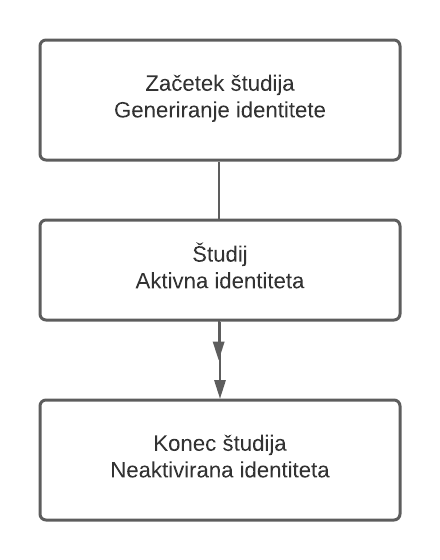
\includegraphics[]{diploma-FRI-vzorec_11maj2021/Blank diagram.png}
\caption{Življenski cikel identitete}
\label{fig:IDlife}
\end{figure}


\section{Življenski cikel identitet za študente}

Za boljše razumevanje bomo definirali naslednje vloge:
\begin{itemize}
    \item Kandidat: Vsaka oseba, ki ima možnost vpisa na študij in se je vpisal na enega izmed študijskih programov.
    \item Študent: Kandidat, ki je bil uspešno vpisan na študijski program. 
    \item Bivši kandidat: Kandidat, ki mu je bil vpis na študijsko smer zavrnjen oz. če kandidat zavrne svoj vpis.
    \item Bivši študent: Študent, ki je bil izključen, se izpiše,nima pogojev za ponavljanje letnika ali dokonča študij.
    
\end{itemize}

Vsaka oseba ima možnost vpisa na študij. V tem trenutku v postopku, bomo to stanje kvalificirali kot \emph{kandidat}. \emph{Kandidat}  je vsak, ki se je vpisal na enega izmed študijskih programov. V tem koraku ima postopek dva možno izida. Prva možnost je, da se \emph{kandidata} sprejme in je uspešno vpisan na študijski program. Če se to zgodi, pridobi vlogo \emph{študent}. Če se to ne zgodi in je zavrnjen pridobi vlogo \emph{ bivšega kandidata}. Enak izid je mogoč, če \emph{kandidat} prekliče svoj vpis. \newline

Ko je \emph{kandidat} vpisan, prejme vlogo \emph{študenta}. V tem stanju \emph{študent} študira. Med študijem je lahko \emph{študent} izključen ali pa se izpiše. Če se to zgodi, pridobi vlogo \emph{bivšega študenta}. Če je uspešen in zaključi letnik oz. diplomira, se mu dodeli vloga \emph{bivši študent}, vsaj je z študijem zaključil. Če ni diplomiral, obstaja možnost, da mora je samo opravil letnik oz. mora ponavljati letnik. V takem primeru se ne zgodi nič (ostane mu vloga \emph{študent}). Če ne izpoljnjuje pogojev za ponavljanje letnika oz. vpis v višji letnik, se študij prekine in dobi vlogo \emph{bivši študent}.

Vsaka oseba, ki je kadarkoli imela vlogo študenta (vse osebe z vlogami \emph{študent} oz. \emph{bivši študent}) imajo na univerzi svojo identiteto. 
Celoten postopek se lahko vidimo na sliki \ref{fig:student}

\begin{figure}[H]
\includegraphics[scale=0.8]{diploma-FRI-vzorec_11maj2021/ID MANAGEMENT ZA ŠTUDENTE.png}
\caption{Upravljanje identitet za študente}
\label{fig:student}
\end{figure}



\section{Trenutno stanje}

Kot sem že omenil v moji motivaciji diplomske naloge ima trenutna implementacija avtentikacije pomanjkljivost. 
\newline 
ID portal za študente je v domeni uni-lj in ima nameščen varnostni certifikat. Iz spletnega naslova lahko ugotovimo, da gre za zaščiteno različico HTTP protokola. Uporabljen je SSL (Secure Sockets Layer) protokol, ki omogoča šifriran prenos informacij prek spleta s protokolom HTTP (Hypertext Transfer Protocol). SSL omogoča uporabo digitalnih certifikatov, tako da spletni brskalnik lahko loči pristno spletno stran aplikacije od lažne. 

Na osnovni strani ID portala za študente lahko študenti upravljajo s svojo identito, med njimi so naslednje možnosti

\begin{itemize}
    \item Aktivacija ali prevzem svoje UL-ID
    \item Sprememba gesla
    \item Urejanje pozabljenega gesla
    \item Preverjanje kombinacije uporabniškega imena in gesla
    \item Prijavljanje napak in težav
\end{itemize}

Pomanjkljivost se nahaja v možnosti urejanja pozabljenega gesla. Celotno zgradbo si lahko preberemo v magistrskem delu Hede Šturm \cite{magistrska}.

\section{Pomanjkljivost}
Leta 2019 sem našel pomanjkljivost v avtentikaciji uporabnikov, če so želeli ponastaviti geslo. Če želimo ponastaviti geslo potrebujemo priskrbeti naslednje podatke:
\begin{itemize}
    \item Ime
    \item Priimek
    \item Uporabniško ime
    \item Datum rojstva
    \item Vpisna številka
    \item Fakulteto
\end{itemize}

Ko priskrbimo podatke se nam novo geslo izpiše na ekran. Če bi želeli ponastaviti geslo, se potrebujemo avtenticirati, kar v preprosti definiciji pomeni, da potrebujemo dokazati da smo oseba, za katero se izdajamo da smo. S tem sistemom to ni mogoče zagotoviti. Poglejmo zakaj.

\begin{itemize}
    \item Ime: Ga ve vsak, ki ga želi vedeti (npr. svojci, na družabnih omrežjih itd.)
    \item Priimek: Ga ve vsak, ki ga želi vedeti (npr. svojci, na družabnih omrežjih itd.)
    \item Uporabniško ime: Ga ne ve vsak, ampak ga ni težko ugotoviti. Uporabniško ime je vezano na osebo in je sestavljeno iz prve črke imena in prve črke priimka, ter štirih številk. Če bi se lotili ugibanja imamo zgolj 10000 možnosti, kar ni veliko.
    \item Datum rojstva: Ga ve vsak, ki ga želi vedeti (npr. svojci, na družabnih omrežjih itd.).
    \item Vpisna številka: Sestavljena iz osmih številk. Prve dve sta šifri fakultete, naslednji dve sta leto vpisa in zadnje štiri so "naključno generirane", ampak lahko z gotovostjo znižamo številko med eno od 0 do 250 (približno število vpisanih dijakov letno na fakulteto).
    \item Fakulteto: Vezana na vpisno številko in pogosto hitro ugotovljena (npr. svojci, družabna omrežja itd.)
\end{itemize}

Vsi podatki, ki jih priskrbimo ne zadostujejo temu, da z gotovostjo potrdijo identiteto osebe, če želi ponastaviti geslo. Ta problem lahko rešimo z dvofaktorsko avtentikacijo, kjer bi uporabnik potreboval še drugo plast avtentikacije (običajno mobilni aparat oz. e-mail naslov ipd.). 

\section{Naše zahteve}

Ker bomo uporavljali z velikim številom uporabniških imen in gesel, bomo potrebovali federacijsko avtentikacijo. S federacijsko avtentikacijo se dostop uporabnikov in preverjanje pristnosti uporavlja centralno. Vse uporabniške identitete se upravljajo v eni bazi podatkov. To omogoča upravitelju omrežja vpogled in vpogled v identitete zaposlenih. Upravitelj omrežja določi podatkovne točke potrebne za ustvarjanje identitet uporabnikov za največjo varnost in natančnost. Federacijska avtentikacija nato temelji na informacijah, ki so na voljo v uporabniški bazi in povezuje to identiteto z digitalnimi dejavnostmi vsakega uporabnika. Poleg tega lahko uporavitelj omrežja nastavijo pravilnike in nadzor kaj, kje in kdaj lahko uporabniki dostopajo do podatkov. Uporabnikom lahko odobrijo ali prekličejo dostop v trenutku, ko se pridružijo drugi skupini ali odidejo na drugo mesto.
\newline

Vse te dodatne plasti varnosti ne povečujejo bremena zaposlenih. Federacijska avtentikacija poenostavi prijavo uporabnikov z odpravo prijavnih pozivov in gesel.

Za določitev identitete uporabnika zadostuje uporabniško ime in geslo. Za uporabnike federacijsko preverjanje pristnosti pomeni manj težav in hitrejši dostop.


\chapter{Potencialne rešitve}

Na slovenskem trgu je več ponudnikov, med njimi QUEST, MS MIM, OSI, LRK, Unistar, IBM in še več.

Ampak nas zanima, če bi lahko univerza sama uredila svojo avtentikacijsko rešitev. Zaradi tega sem si pogledal odprtokodne rešitve. Med njimi so naslednji, kot so Authentik, Keycloak, Authelia...


\subsection{Možnost 1 - Authentik}

Od prej naštetih odprtokodnih rešitev (Authentik, Keycloak, Authelia) si bomo najprej pobližje pogledali Authentik. 

V dokumentaciji Authentika\cite{AuthentikLink} lahko vidimo, da bomo za namestitev potrebovali docker, docker-compose ter Linux sistem, na katerem bomo gostili Authentik. Docker in docker-compose sta javno dostopna in brezplačna. 
\newline    
Authentik, kot ponudnik identitete, podpira SAML2, 0Auth2, OIDC in LDAP. Ker bomo potrebovali federacijsko avtentikacijo mora naš ponudnik identete podpirati SAML, za kar je pa Authentik ustrezen. 

Authentik omogoča tudi registracijo uporabnikov, če bi se za to odločili. Prav tako imamo popoln dostop do vseh funkcionalnosti kar nam omogoča, da lahko sami odpravimo probleme, ki se pojavijo in nam ni treba čakati na posrednika. Podpira tudi večkratno preverjanje pristnosti, kar nam poveča varnost uporabnikov. 
\newline    
Meni najboljša lastnost je pa aktivna baza uporabnikov in razvijalcev, ki so dostopni na Discord serverju, ki je dostopen tudi preko uradne strani Authentika: \url{https://discord.com/invite/jg33eMhnj6}

\subsection{Možnost 2 - Keycloak}

Keycloak je po zmožnostih zelo podoben Authentiku. 

Prav tako podpira SAML2, OAuth2 in OIDC. Ne podpira protokola LDAP, ampak ga v nimamo v našem načrtu. 
\newline
Uporabniki se prav tako lahko registrirajo in imamo popoln dostop do funkcionalnosti. Podpira večkratno preverjanje pristnosti.

Razlog, da smo izbrali Authentik in ne Keycloak je, ker imamo boljši dostop do skupnosti razvijalcev in uporabnikov pri Authentiku.

\subsection{Možnost 3 - Authelia}

V industriji je od 2016 in je uporabniku prijazna, ampak za nas ni primerna. 
\newline
Za naše potrebe ne podpira protookla SAML2 ali OAuth2, kar je za nas ključnega pomena, zato za nas ni primerna. 

\section{Arhitektura sistema}

Sedaj ko vemo kaj potrebujemo lahko začnemo z zgradbo sistema. Potrebovali bomo ponudnika identitete, ki vzpostavi identiteto uporabnika in se poveže s ponudnikom storitev. Nato pa varnostni protokol SAML (Security Assertion Markup Language) preveri pristnost uporabnika. 

Izbrati moramo ponudnika identitete, ki nudi podporo federacijam, ter podpira protokol SAML. Od že prej naštetih (Authentik,Keycloak, Apache Syncope, FusionAuth, OpenIAM, Gluu ipd.) sem izbral Authentik. Je brezplačen, odprtokoden ter ima aktivno bazo uporabnikov ter razvijalcev. Seveda nudi tudi podporo vsem že naštetim zahtevam.  
\newline

Authentik sem postavil na Ubuntu Serverju ter vzpostavil par testnih uporabnikov. Za ponudnika storitve sem vzpostavil Wordpress stran na spletni strani www.davidkonc.xyz (dostopno: 23.5.2022). Uporabnik lahko bere blog, ter ureja nastavitve, ampak da lahko ureja nastavitve se more prijaviti. Za prijavo se uporabnika preusmeri na Authentik, kjer se avtenticira in potem lahko ureja stran. 

\begin{figure}[H]
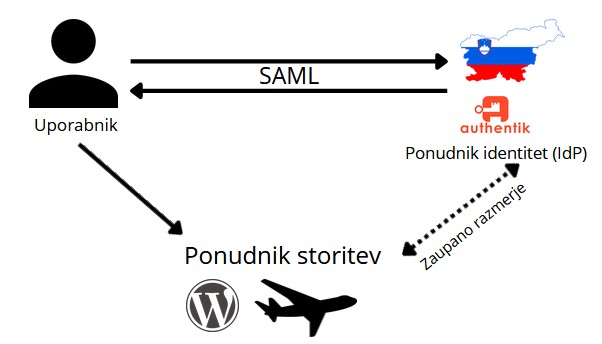
\includegraphics[scale=0.7]{diploma-FRI-vzorec_11maj2021/SAML.jpg}
\caption{Kako deluje SAML}
\label{fig:grafMoj}
\end{figure}

 \section{Namestitev Authentika}

Uspešna namestitev Authentika ima par zahtev, ki jih lahko vidimo na spletni strani \cite{AuthentikLink}.
Potrebovali bomo operacijski sistem Linux z vsaj dvema jedroma in vsaj 2GB RAM-a. Poleg tega bomo potrebovali docker, ter docker-compose. 

Docker je odprtokodna tehnologija kontejnerizacije za gradnjo in posodabljanje naših aplikacij.
Docker compose je orodje za definiranje in izvajanje aplikacij Docker z več kontejnerji. Z možnostjo Compose uporabimo datoteko YAML za konfiguriranje storitev naših aplikacij. Nato z enim ukazom ustvarimo in zaženemo vse storitve iz naših konfiguracij.
\subsection{Namestitev Docker in docker-compose}

Za namestitev docker na sistemu Ubuntu lahko sledimo uradni strani \cite{DockerLink}, ki nam pove kaj vse moramo storiti. 

Najprej bomo odstranili stare verzije, če so prisotne. Če pa niso, nam pa zagnati tak ukaz ne škodi.


\begin{lstlisting}[language=bash]
 $ sudo apt-get remove docker docker-engine docker.io containerd runc
\end{lstlisting}

 Nato pa lahko naložimo Docker. Obstaja več možnih načinov, mi bomo uporabili curl.
 \newline
 Ukaz curl je orodje za prenos ali prenos datotek/podatkov iz ali na strežnik z uporabo FTP, HTTP, HTTPS, SCP, SFTP, SMB in drugih podprtih protokolov v sistemu Linux ali Unixu.
 
 Če še nimamo nameščenega na sistem, ga moramo naložiti z uporabo apt ukaza oz. apt-get ukaza. To lahko naredimo preprosto z naslednjimi ukazi.
 
\begin{lstlisting}[language=bash]
$ sudo apt update
$ sudo apt upgrade
$ sudo apt install curl
\end{lstlisting}

Sedaj lahko namestimo docker z naslednjima ukazoma.


\begin{lstlisting}[language=bash]
$  curl -fsSL https://get.docker.com -o get-docker.sh

$  sudo sh get-docker.sh
\end{lstlisting}

Od zahtev za namestitev Authentika nam sedaj manjka samo še Docker Compose. Navodila za njegovo namestitev lahko najdemo na spletni strani \cite{DockerCompose}. 

Namestili ga bomo ponovno z uporabo ukaza curl, ki ga sedaj že imamo nameščenega.


\begin{lstlisting}[language=bash]
$ curl -SL https://github.com/docker/compose/releases/
download/v2.5.0/docker-compose-linux-x86_64 -o /
usr/local/bin/docker-compose

$   sudo chmod +x /usr/local/bin/docker-compose
\end{lstlisting}

Če nam je namestitev uspela, lahko preverimo verzijo Docker Compose, z naslednjim ukazom. Če se nam verzija prikaže, je namestitev uspela.

\begin{lstlisting}[language=bash]
$  docker-compose --version
\end{lstlisting}

\subsection{Namestitev sistema}

Ko imamo vse potrebne zahteve za namestitev sistema, lahko začnemo z namestitvijo. Kot sem omenil pri Docker Compose, bomo za konfiguracijo sistema uporabili datoteko YAML. Datoteko YAML lahko dobimo na spletni strani od Authentika\cite{AuthentikYAML} in jo postavimo v direktorij, kjer želimo imeti naš projekt. 

Docker-compose projekt vsebuje naslednje kontejnerje:

\begin{itemize}
    \item Server. To je zaledna storitev, ki izvaja vso logiko, izvaja API in dejanski del SSO. Prav tako poganja sprednji del, gosti datoteke JS/CSS in služi tudi datotekam, ki smo jih naložili za ikone/itd.
    \item Worker. Ta kontejner izvaja opravila v ozadju, vse, kar lahko vidite na strani Sistemska opravila v sprednjem delu.
    \item redis in postgresql. Predpomnilnik in baza podatkov.
\end{itemize}

Ker je to sveža namestitev Authentika, moramo še zgenerirati geslo. V ukaznem pozivu se premaknemo v direktorij, kamor smo shranili prej omenjeno YAML datoteko. Sedaj pa napišemo naslednje ukaze.

\begin{lstlisting}[language=bash]
$  sudo apt-get install -y pwgen
echo "PG_PASS=$(pwgen -s 40 1)" >> .env
echo "AUTHENTIK_SECRET_KEY=$(pwgen -s 50 1)" >> .env
\end{lstlisting}

Zaradi omejitve PostgreSQL so podprta gesla samo do 99 znakov. Več o tem si lahko preberete na uradni strani od PostgreSQL\cite{PostgreSQL}. Kljub temu bo to nam zadostovalo. \newline

V .env datoteki v našem direktoriju se trenutno nanaša naše geslo. Poleg tega, lahko v .env datoteko dodamo še par vrstic, da bo Authentik tekel na bolj prepoznavnih vratih 80/443. Da to naredimo, vse kar rabimo narediti, je dodati 2 vrstici kode na konec datoteke .env.

\begin{lstlisting}[language=bash]
AUTHENTIK_PORT_HTTP=80
AUTHENTIK_PORT_HTTPS=443
\end{lstlisting}

Sedaj poženemo še naslednji ukaz, da se naše spremembe uveljavijo. 

\begin{lstlisting}[language=bash]
$ sudo docker-compose up -d
\end{lstlisting}

Da dokončamo nastavitev nam manjkata samo še dva ukaza, ki bosta sistem tudi zagnala.

\begin{lstlisting}[language=bash]
$ sudo docker-compose pull
$ sudo docker-compose up -d
\end{lstlisting}

Naš sistem je postavljen. Da začnemo z upravljanjem našega sistema, navigiramo na naslov: $$https://<serverIP>/if/flow/initial-setup/$$. $$<serverIP>$$ moramo zamenjati z IP naslovom našega Ubuntu serverja. To lahko naredimo tako, da v ukazni poziv vpišemo naslednji ukaz:
\begin{lstlisting}[language=bash]
ip addr show
\end{lstlisting}

\begin{figure}[H]
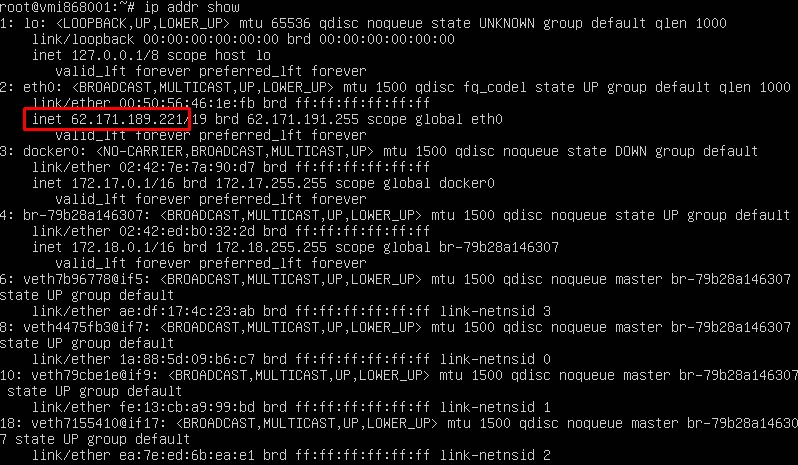
\includegraphics[scale=0.75]{diploma-FRI-vzorec_11maj2021/IP naslov.jpg}
\caption{Naš IP naslov}
\label{fig:student}
\end{figure}

Iz dobljenega razberemo naš IP naslov, ter z njim zamenjamo značko $$<serverIP>$$. To nas potem prinese na stran, kjer moramo določiti geslo za administratorja. 

\begin{figure}[H]
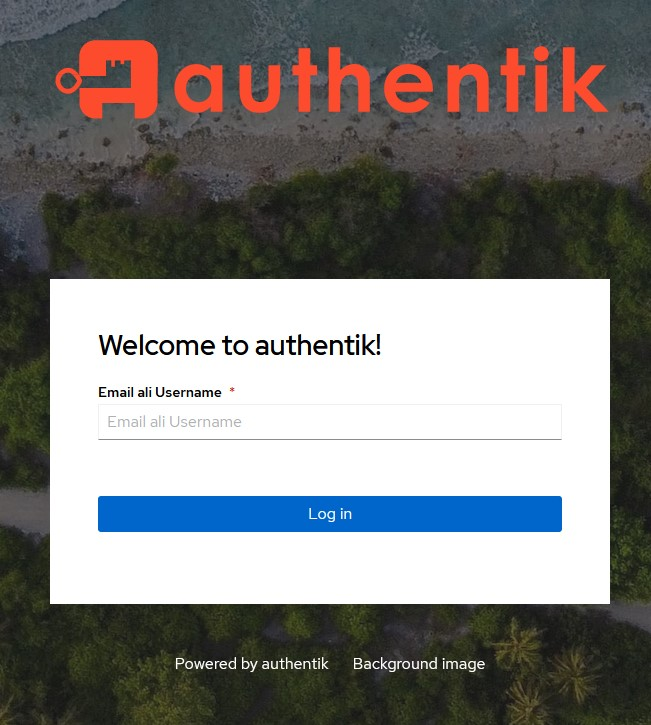
\includegraphics[scale=0.75]{diploma-FRI-vzorec_11maj2021/Uvodna stran.jpg}
\caption{Prijavna stran}
\label{fig}
\end{figure}


\section{Namestitev ponudnika storitev}

Za ponudnika storitev sem se odločil, da bom gostil spletno stran Wordpress. Uporabniki se bodo lahko prijavili v spletno stran, ter posledično urejali izgled, pisali objave, upravljali nastavitve ipd. 
Neprijavljeni uporabniki bodo pa lahko samo brali objave. 
\newline
Pri namestitvi Wordpressa bo veliko lažje, ker sem že pred pisanjem diplomskega dela imel v lasti svojo domeno, ki jo gostim preko hostinger.com in je dostopna na \href{www.davidkonc.xyz}{www.davidkonc.xyz} (dostopano 30.05.2022). 
\newline
Spletna stran je uporabniku prijazna, ima namreč veliko pripomočkov, ki nam bodo pri delu prišli prav.
Preko uporabniškega vmesnika lahko registriramo domeno. Jaz sem si izbral ime davidkonc.xyz, ker sem ga uporabljal za online življenjepis pred pisanjem mojega diplomskega dela. 
\newline
Ko imamo registrirano domeno, lahko kliknemo na gumb "Manage", ki nas bo nesla na meni, ki upravlja z našo spletno stranjo, kot je to videno na sliki \ref{fig:hostinger}.

\begin{figure}[H]
\hspace{-3,5cm}
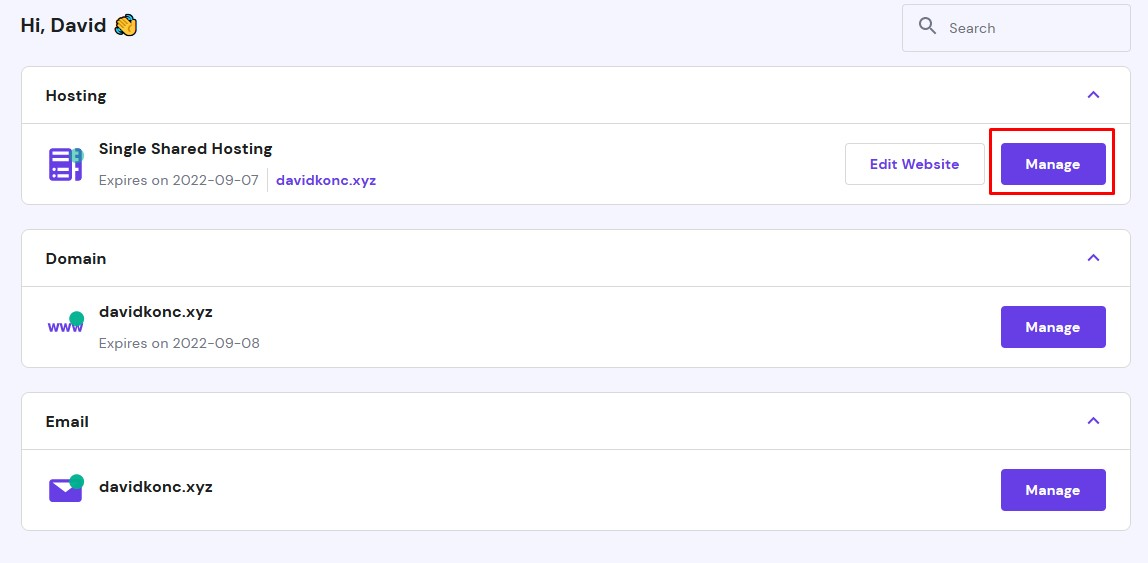
\includegraphics[scale=0.65]{diploma-FRI-vzorec_11maj2021/hostinger.jpg}
\caption{Uporabniški vmesnik Hostinger.com}
\label{fig:hostinger}
\end{figure}


Gumb nas preusmeri na upravljalno ploščo naše spletne strani. Na njej lahko vidimo gumb "Install Wordpress", ki nam bo sam namestil Wordpress vmesnik na našo spletno stran. Če po tem dejanju dostopamo na našo spletno stran (\href{www.davidkonc.xyz}{www.davidkonc.xyz}) je sedaj viden osnoven Wordpress blog, kot vidno na sliki \ref{fig:wordpressOsn}.

\begin{figure}[H]
\hspace{-4cm}
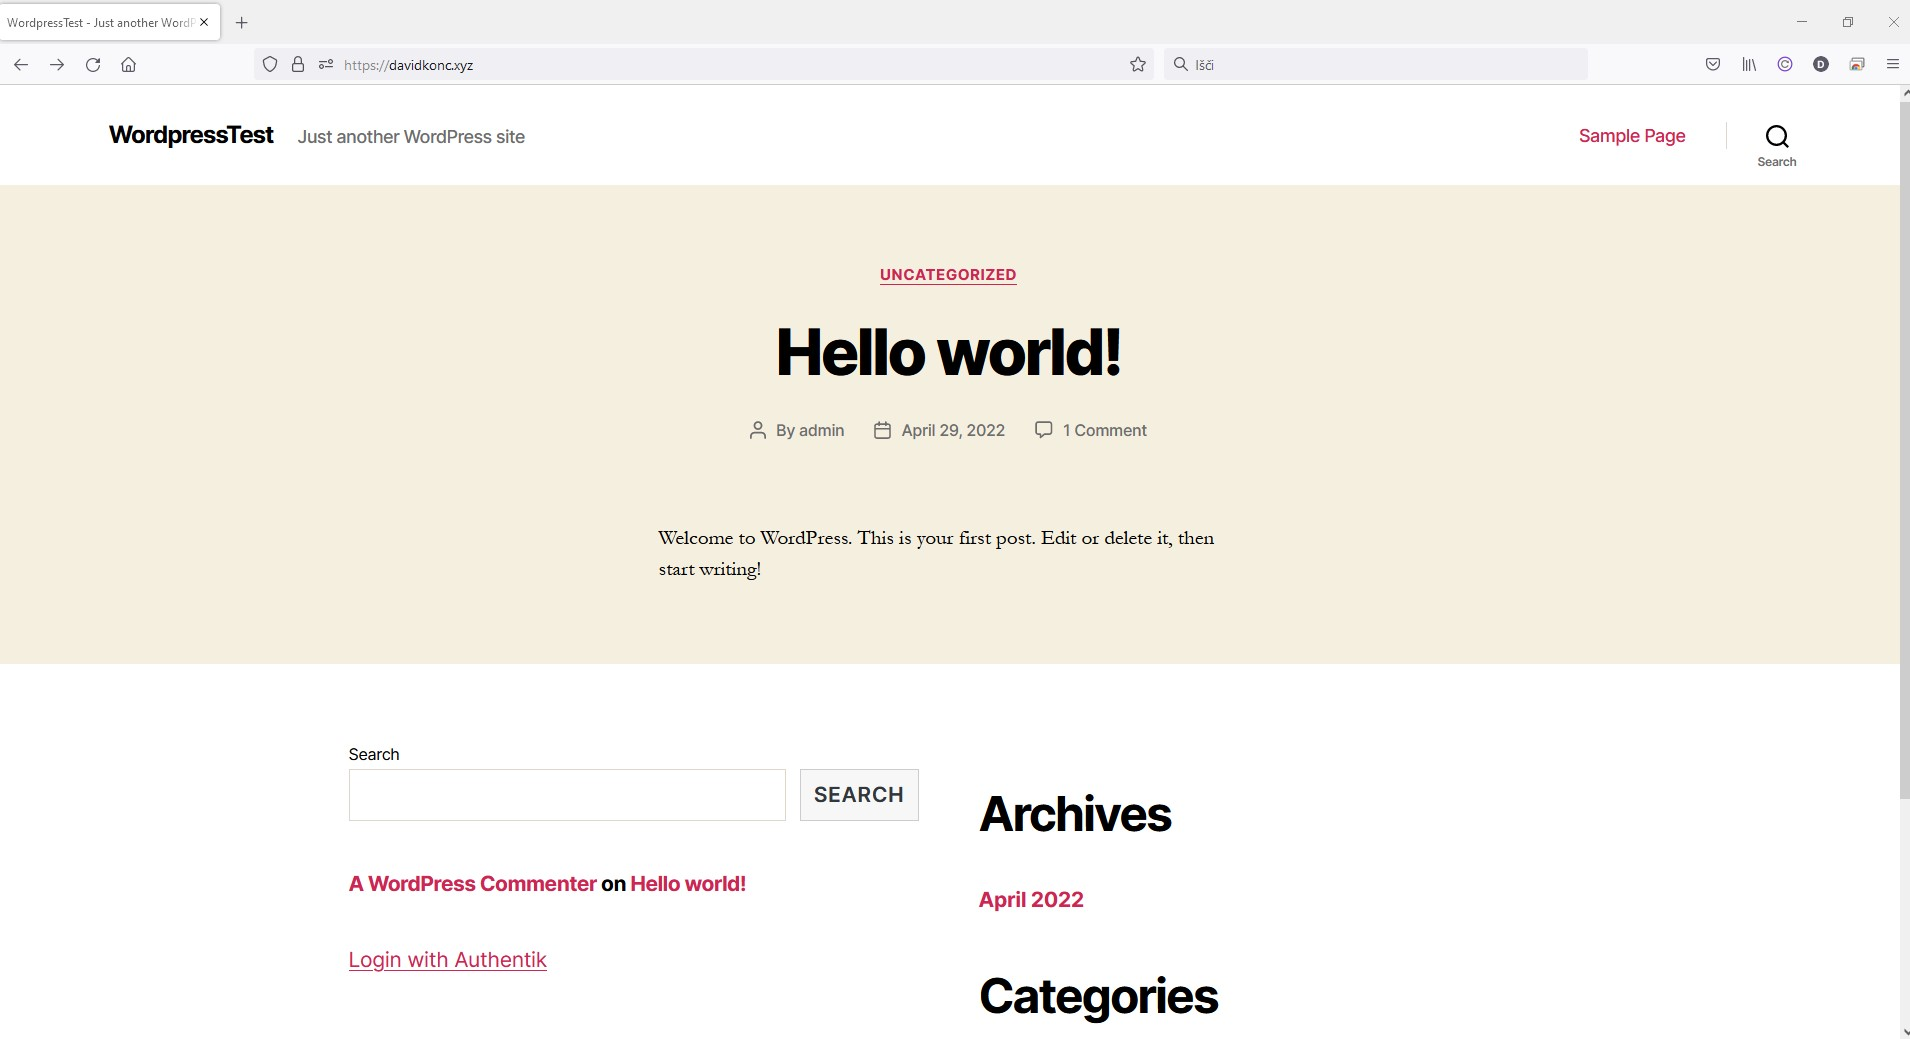
\includegraphics[scale=0.50]{diploma-FRI-vzorec_11maj2021/wordpress.jpg}
\caption{Spletna stran davidkonc.xyz po namestitvi Wordpress vmesnika}
\label{fig:wordpressOsn}
\end{figure}



\subsection{Upravljanje Wordpress strani}

Sedaj, ko imamo nameščeno spletno stran jo lahko začnemo urejati, da bo primerna za našo potrebo povezave z Authentikom. Ob naložitvi Wordpressa na našo spletno stran, se je tudi kreiral administratorski uporabnik, ki ima enako ime in geslo kot uporabnik do našega gostitelja storitve. Da se prijavimo v našo storitev gremo lahko na spletno stran \href{www.davidkonc.xyz/wp-admin/}{www.davidkonc.xyz/wp-admin/}, ter se prijavimo.
\newline
Prijavljeni smo v administratorsko konzolo, kot je videno na sliki \ref{fig:adminWord}.

\begin{figure}[H]
\hspace{-2cm}
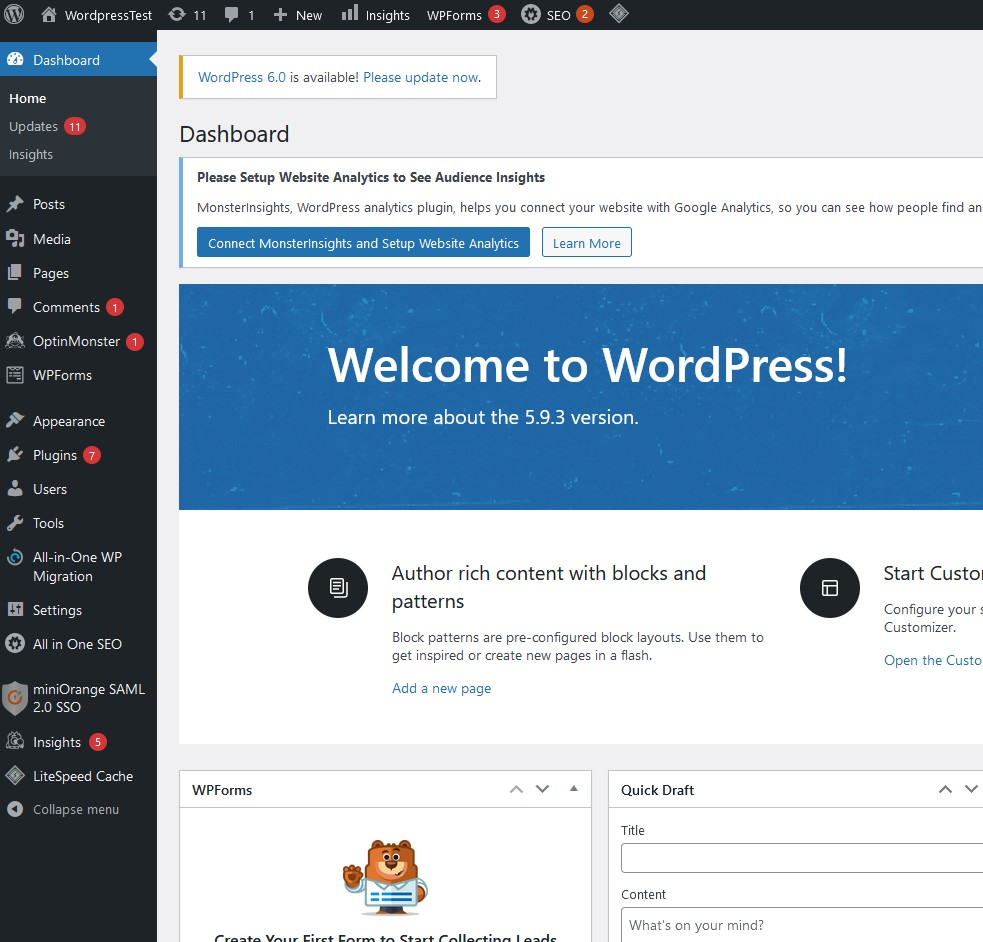
\includegraphics[scale=0.7]{diploma-FRI-vzorec_11maj2021/Screenshot_1.jpg}
\caption{Administratorska konzola Wordpress}
\label{fig:adminWord}
\end{figure}

\section{Povezovanje Wordpressa z Authentikom}

Cilj naloge je pridobiti možnost vpisa v našo administratorsko konzolo preko Authentika. Kot že omenjeno v poglavju Naše zahteve bomo potrebovali podporo federacijam, da se lahko veliko uporabnikov prijavi z uporabniškim imenom in geslom federacije. To lastnost podpira protokol SAML.

\subsection{O SAML-u}

\subsubsection{Kaj je SAML?}
SAML je akronim, ki se uporablja za Security Assertion Markup Language. Je odprt standard, ki se uporablja za preverjanje pristnosti. Njegova primarna vloga pri spletni varnosti je, da nam omogoča dostop do več spletnih aplikacij z enim parom uporabniškega imena in gesla za prijavo. Deluje tako, da posredujemo podatke za preverjanje pristnosti v določeni obliki med dvema strankama, običajno ponudnikom identitete (idP), kar je v našem primeru Authentik in spletno aplikacijo, kar je v našem primeru Wordpress.
Spletne aplikacije na podlagi formata Extensible Markup Language (XML) uporabljajo SAML za prenos podatkov za preverjanje pristnosti.
\newline
Tehnološka industrija je ustvarila SAML za poenostavitev postopka preverjanja pristnosti, kjer so uporabniki morali dostopati do več neodvisnih spletnih aplikacij v različnih domenah. Ta lastnost je za nas glavna, ker ravno to je eden glavnih lastnosti, da ga bomo uporabili. Želimo, da če se želimo vpisati v e-mail račun lahko uporabimo enako uporabniško ime in geslo, kot pa če se želimo prijaviti v spletno učilnico. 

\subsubsection{Kako deluje SAML?}
SAML deluje tako, da izmenjuje uporabniške podatke, kot so prijave, stanje preverjanja pristnosti, identifikatorji in drugi ustrezni atributi med identiteto in ponudnikom storitev. Posledično se poenostavi in zavaruje postopek preverjanja pristnosti, saj se mora uporabnik prijaviti samo enkrat z enim samim parom uporabniškega imena in gesla za preverjanje pristnosti. Torej, ko uporabnik poskuša dostopati do spletnega mesta, ponudnik identitete posreduje preverjanje pristnosti SAML ponudniku storitev, ki nato odobri vnos uporabnika. Da bomo razumeli bolje, lahko uporabimo analogijo iz resničnega sveta.
\newline
Dober primer je letalska industrija. Preden se vkrcate na letalo, mora letalski prevoznik potrditi, da smo tisti, za katerega se predstavljamo, da zagotovi varnost drugih potnikov. Torej preverijo našo identiteto z neko obliko identifikacije s sliko, ki jo je izdal državni organ. Ko potrdijo, da se vaše ime na naši identiteti ujema z imenom na naši letalski vozovnici, nam nato dovolijo, da se vkrcamo na letalo.
\newline
V spodnji sliki \ref{fig:grafMoj} je država ponudnik identitete, letalska družba pa ponudnik storitev. Naša identifikacijska številka, ki jo je izdal državni organ, je trditev SAML. Ko zaprosimo za osebno izkaznico, moramo običajno izpolniti obrazec, se fotografirati in v nekaterih okoliščinah tudi oddati prstne odtise. Država (ponudnik storitev) nato te identifikacijske atribute shrani v svojo bazo podatkov in nam izda fizični ID, povezan z našo identiteto. V primeru letalske družbe, ko prispemo do izhoda, letalska družba (ponudnik storitev) preveri našo trditev ID (SAML). Letalska družba sprejme našo osebno izkaznico, saj vsebuje naše podatke, osebna izkaznica ali potni list pa se pregleda kot veljaven dokument. Po uspešni avtentikaciji nam letalska družba dovoli vkrcanje na letalo.

\subsubsection{Postopek avtentikacije z uporabom SAML-a}

SAML uporablja potek dela za preverjanje pristnosti, ki temelji na zahtevkih. Prvič, ko uporabnik poskuša dostopati do spletnega mesta, ponudnik storitev od ponudnika identitete zahteva, da preveri pristnost uporabnika. Nato ponudnik storitev uporabi trditev SAML, ki jo je izdal ponudnik identitete, da uporabniku odobri dostop. Ponazorimo potek dela s primerom.

\begin{itemize}
    \item Uporabnik odpre svoj brskalnik in se pomakne do spletne aplikacije ponudnika storitev, ki za preverjanje pristnosti uporablja ponudnika identitete.
    \item Spletna aplikacija se odzove z zahtevo SAML.
    \item Brskalnik posreduje zahtevo SAML ponudniku identitete.
    \item Ponudnik identitete razčleni zahtevo SAML.
    \item Če uporabnik ni overjen potem ponudnik identitete preveri pristnost uporabnika tako, da zahteva uporabniško ime in geslo ali kakšen drug faktor avtentikacije. Če je uporabnik že overjen, potem ponudnik identitete ta korak preskoči.
    \item Ponudnik identitete generira odgovor SAML in ga vrne v uporabnikov brskalnik.
    \item Brskalnik pošlje ustvarjen odgovor SAML spletni aplikaciji ponudnika storitev, ki ga preveri.
    \item Če je preverjanje uspešno, spletna aplikacija uporabniku odobri dostop.
\end{itemize}
    
\subsection{Implementacija SAML-a}

Ker imamo za ponudnika storitev Wordpress, se lahko poslužimo enega izmed mnogih vtičnikov, ki bo naredil SAML implementacijo za nas enostavno.  

V zavihku Plugins (vtičniki) izberemo možnost Add new (dodaj novo). Če v okno za iskanje vnesemo besedo ''SAML'', se nam prikaže vtičnik  ''SAML Single Sign On - SAML SSO Login'', ki ga je naredilo podjetje miniOrange\cite{miniOrange}. 
\newline
Ko ga namestimo, se nam prikaže nov meni z imenom ''miniOrange SAML 2.0 SSO''. Ta meni in meni v Authentiku bomo sedaj uporabili, da vzpostavimo avtentikacijo. 
\newline
Najprej pojdimo v Authentik meni, da najprej naredimo aplikacijo na ponudniku identitet. Navigiramo na IP-naslov našega ponudnika in se vpišemo z uporabniškim imenom administratorja, ki smo ga nastavili, ko smo nameščali Authentik. Ko se prijavimo, lahko vidimo, da še nimamo aktivnih aplikacij. Navigiramo na "Admin interface" (skrbniški vmesnik), kjer lahko sedaj na levi strani v meniju vidimo vse možnosti.

\begin{figure}[H]
\hspace{-3cm}
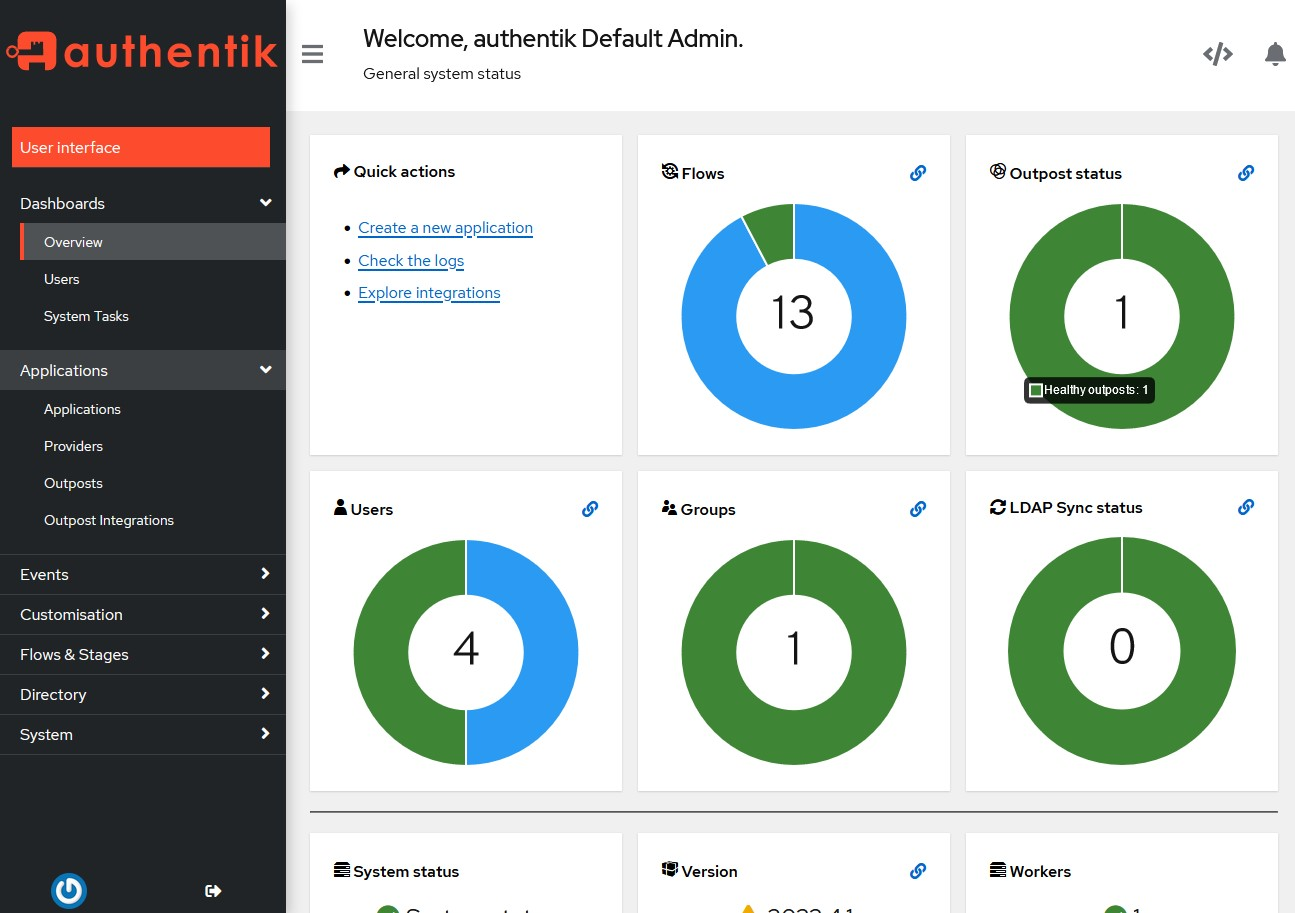
\includegraphics[scale=0.55]{diploma-FRI-vzorec_11maj2021/admin_inter.jpg}
\caption{Skrbniški vmesnik Authentika}
\label{fig}
\end{figure}

Izberemo možnost Applications in Create, tukaj moramo pa sedaj specificirati vse potrebno, za uspešno povezavo. Tu je pomembno okno Provider (ponudnik), ki ga moramo tudi narediti. To bo naša implementacija SAML-a.Lahko kar kliknemo gumb Create provider (naredi ponudnika) in izberemo možnost ''SAML Provider''. 
Od nas se bodo zahtevali naslednji podatki in vnesli bomo naslednje:
\begin{itemize}
    \item Name (ime): Wordpress (izberemo sami).
    \item Authorization flow: default-provider-authorization-explicit-consent
    \item ACS URL: ta podatek pridobimo na strani vtičnika na naši Wordpress strani - v našem primeru je to: https://davidkonc.xyz/
    \item Issuer: ta podatek pridobimo na strani vtičnika na naši Wordpress strani - v našem primeru je to: https://davidkonc.xyz/wp-content/plugins/miniorange-saml-20-single-sign-on/
    \item Service Provider Binding:  Post
\end{itemize}

\begin{figure}[H]
\hspace{-1cm}
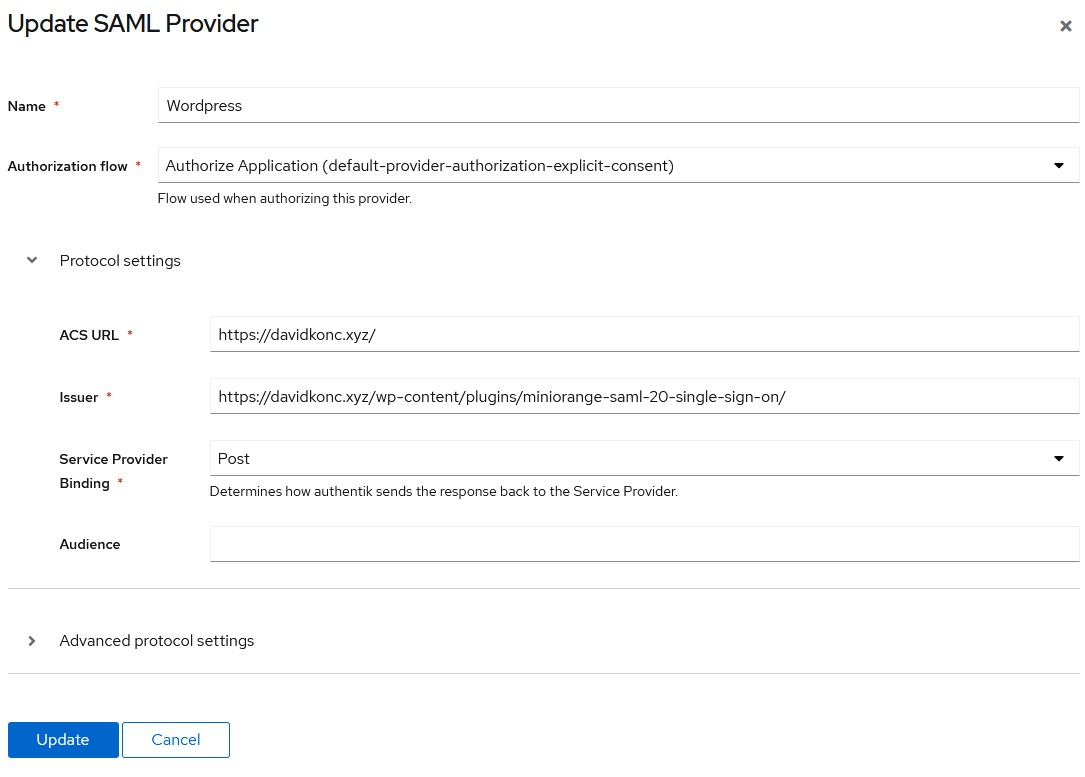
\includegraphics[scale=0.6]{diploma-FRI-vzorec_11maj2021/SAMLprovi.jpg}
\caption{Okno z nastavitvami ponudnika v Authentiku}
\label{fig}
\end{figure}

\begin{figure}[H]
\hspace{-4cm}
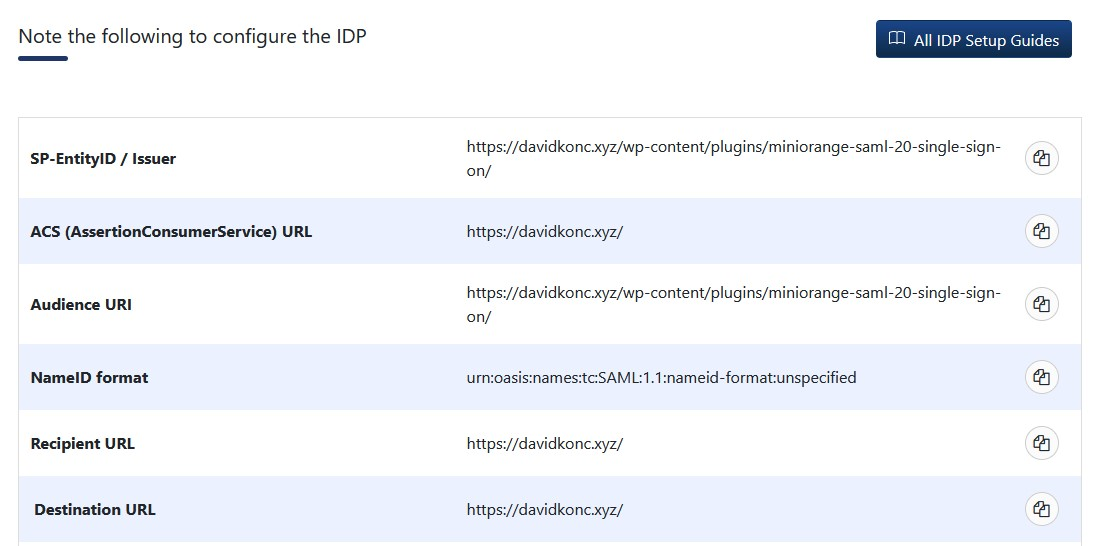
\includegraphics[scale=0.7]{diploma-FRI-vzorec_11maj2021/WordpressSAML.jpg}
\caption{Okno z lastnostmi v SAML vtičniku v Wordpressu}
\label{fig}
\end{figure}

Ko imamo ustvarjeneva ponudnika (Provider) v Authentiku, lahko dokončamo ustvarjanje aplikacije. Izpolniti moramo naslednje možnosti:
\begin{itemize}
    \item Name (ime): Wordpress (izberemo sami).
    \item Slug: Wordpress (izberemo sami).
    \item Provider: Wordpress (ime od pravkar ustvarjenega ponudnika).
    \item Policy engline mode: ANY, any policy must match to grant access (privzeta vrednost). 
\end{itemize}

\begin{figure}[H]
\hspace{-2cm}
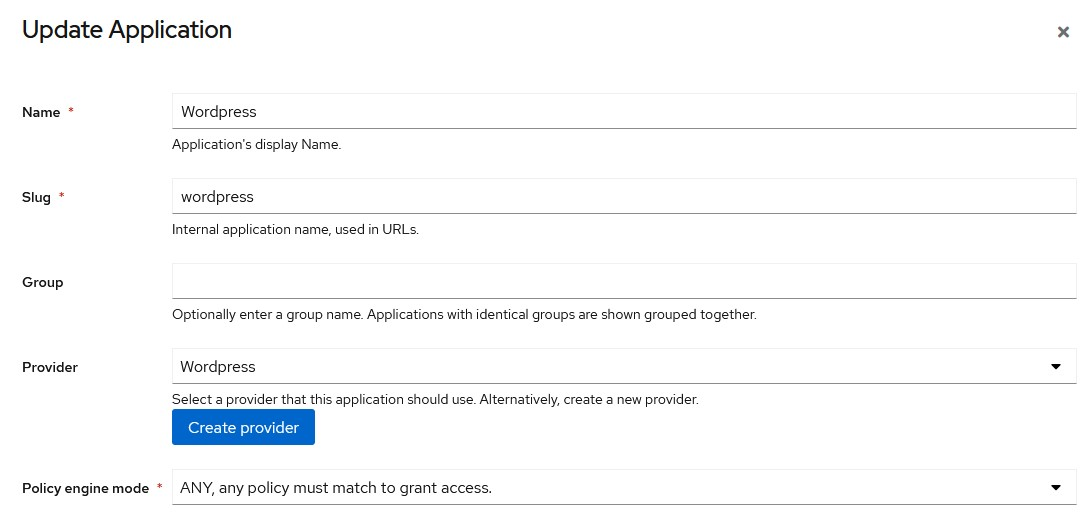
\includegraphics[scale=0.65]{diploma-FRI-vzorec_11maj2021/AuthAplication.jpg}
\caption{Okno z nastavitvami aplikacije v Authentiku}
\label{fig}
\end{figure}

Sedaj smo na strani Authentika opravili. Konfigurirajmmo še vtičnik v Wordpressu. V meniju vtičnika izberemo ''Service Provider Setup'' in izberemo možnost ''Upload IDP Metadata''. Tukaj moramo sedaj vnesti XML datoteko z metapodatki od našega ponudnika identitet. To lahko dobimo pri našem ponudniku identitet v zavihku ''Provider'', kjer izberemo ponudnika, ki smo ga mi kreirali in ga izberemo. Na dnu strani se nam pojavi veliko okno z vsemi metapodatki. To lahko prenesemo, da potem naložimo v vtičnik v Wordpressu. 

\begin{figure}[H]
\hspace{-4cm}
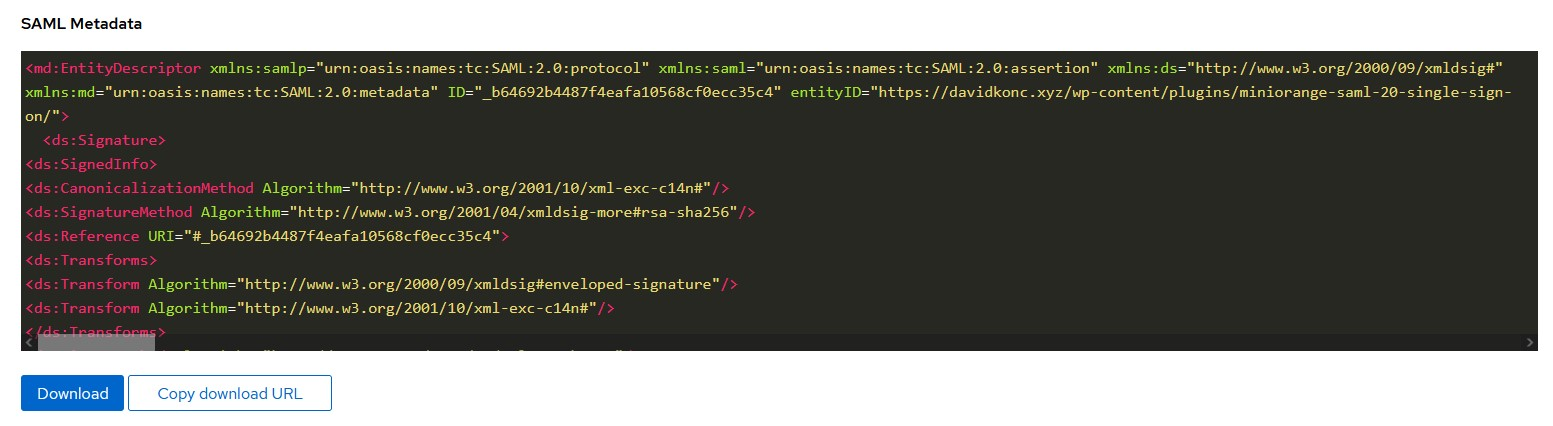
\includegraphics[scale=0.5]{diploma-FRI-vzorec_11maj2021/SAMLMetadata.jpg}
\caption{Metapodatki v Authentiku}
\label{fig}
\end{figure}

\subsection{Test konfiguracije}

Z implementacijo smo sedaj zaključili. Preverimo, če sedaj vse deluje kot mora. 
To bomo naredili na naslednji način:
\begin{itemize}
    \item Navigirali bomo na prijavno stran od Wordpressa, ter se poskusili prijaviti z našim administratorskim uporabniškim imenom in geslom (od Authentika). 
    \item Če je prijava uspešna bomo ustvarili novega uporabnika v direktoriju uporabnikov v Authentiku, brez vseh pravic. 
    \item Navigirali bomo na prijavno stran od Wordpressa, ter se poskusili prijaviti z uporabniškim imenom in geslom od novo ustvarjenega uporabnika. Če je prijava uspešna, implementacija deluje. 
\end{itemize}

Navigirajmo na prijavno stran od Wordpressa, kjer sedaj lahko opazimo gumb ''Login with Authentik''. To bo sedaj naša izbira prijave. 


\begin{figure}[H]
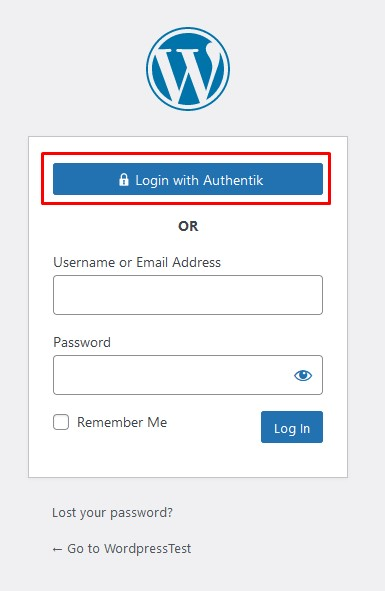
\includegraphics[scale=0.9]{diploma-FRI-vzorec_11maj2021/WordpressLOGIN.jpg}
\caption{Prijavna stran v Wordpressu z novo možnostjo prijave}
\label{fig}
\end{figure}

Ko pritisnemo ta gumb nas preusmeri na stran Authentika, kjer sedaj vpišemo uporabniško ime in geslo administratorja. Če je prijava uspešna lahko sedaj vidimo administratorski pogled z vsemi možnostmi v meniju. 
\newline
To nam je uspelo. Sedaj moramo ustvariti novega uporabnika v Authentiku. V Authentiku navigirajmo v direktorij ''Users'' (uporabniki), kjer lahko ustvarimo novega uporabnika s pritiskom gumba ''Create'' (ustvari). Vse kar potrebujemo je uporabniško ime, ki si ga izberemo, v tem primeru bomo izbrali ime ''student''. Ko smo ga ustvarili, kliknemo na novo ustvarjenega uporabnika, ter izberemo možnost ''Set password'' (nastavi geslo). Izberemo geslo.  
\newline
Ko smo vse to naredili ponovimo postopek prijave. Navigiramo na prijavno stran, vnesemo uporabniško ime in geslo in če vidimo administratorski prikaz, nam je uspelo. 
\newline

\chapter{Zaključek}

V tem diplomskem delu smo razvili novo avtentikacijsko rešitev za potencialno uporabo na Univerzi v Ljubljani. Vzpostavili smo ponudnika identitete Authentik, ki je odprtokoden in sicer na naš Ubuntu Serverju. Vzpostavili smo ponudnika storitev, ki bo potreboval avtentikacijo. Za to nalogo smo izbrali Wordpress, zaradi vnaprej ponujenih vtičnikov, ki so nam olajšali delo. Za povezavo med njima pa smo izbrali protokol SAML, ki podpira federacijsko avtentikacijo, da lahko uporabnikom omogočimo preprostejšo prijavo na več storitev. 
\newline
S tem sistemom odpravimo pomanljkjivost, ker ob kreaciji uporabnikov, priskrbimo pomožne e-mail naslove, na katere se pošlje ponastavljena gesla. 
\newline
Sestava sistema nam je uspela in smo se uspešno prijavili v Wordpress (ponudnik storitve) s tem, da smo se avtenticirali pri našem ponudniku identitete (Authentik). 
\newline
Ampak žal naša rešitev ni brez pomankljivosti. Najbolj pogosti dve pomanjkljivosti nista odpravljeni s federacijsko avtentikacijo. To so notrajnje grožnje in kraja identitete. Biti moramo popolnoma prepričani v zanesljivost uporabnikov v omrežju in imeti protokole za preverjanje pristnosti zasnovane tako, da zagotovijo, da je vsak uporabnik tisti, za katerega trdi, da je. Izobraževanje uporabnikov je potrebno za zmanjšanje tveganja človeške napake, saj lahko en sam ogrožen par federacijskih poverilnic hekerjem omogoči dostop do več aplikacij in omogoči hitro širjenje kršitve po omrežju.
Nepravilna oskrba, ki vodi do prekoračitve privilegijev, lahko pusti odprta vrata za kršitve. Uporabnikova združena identiteta bi morala omogočati le raven dostopa, ki je potrebna za njegovo ali njeno delo in vsak začasni dostop, potreben za kratkoročne projekte, je treba preklicati takoj, ko ni več potreben. Avtomatizirane rešitve za odobritev in preklic dostopa postajajo vse pogostejša.
\newline
Našo rešitev bi lahko nadgradili tako, da bi vzpostavili sistem skupin, kjer bi vsakega uporabnika uvrstili v primerno skupino in potem prirejali pravice skupinam. To bi bil najlažji sistem vzdrževanja pravic uporabnikom, ker jim bi bilo potrebno samo določiti vlogo v sistemu. Tako bi potem uporabniki imeli dostop do aplikacij, ki so vezani na to vlogo. 
\newline
Za zaključek bi dodal, da čeprav ni naša rešitev brez napak, odpravlja glavne pomanjkljivosti avtentikacije, ki bi nam olajšale prijavo, s tem pa bi bolje zavarovali sistem. 


\cleardoublepage
%\addcontentsline{toc}{chapter}{Literatura}

\printbibliography[heading=bibintoc,type=article,title={Članki v revijah}]

\printbibliography[heading=bibintoc,type=inproceedings,title={Članki v zbornikih}]

\printbibliography[heading=bibintoc,type=incollection,title={Poglavja v knjigah}]

\printbibliography[heading=bibintoc,title={Celotna literatura}]


\end{document}

